\section{Datasets}

Labeled data has a crucial influence on algorithm development and evaluation in
research fields dealing with classification and detection. Any machine learning algorithm is only as good as the data behind it in terms of modeling and generalization
properties.

Well-established and easily accessible benchmark databases attract the
interest of the research community as readily available support for research, thus
 accelerating the pace of development for related fields. There are many well-known
databases in related research areas, such as TIMIT \cite{garofolo1993darpa} for speech
recognition or the Million Song Dataset \cite{bertin2011million} for various tasks in
music information retrieval. In view of this critical influence, the process of creating
a dataset for system developing is, naturally, very delicate. The content must be carefully
selected to provide sufficient coverage of the aspects of interest, sufficient variability
in characterizing these aspects, and a sufficient quantity of examples for robust
modeling. Unfortunately, there is no rule on what ``sufficient'' means, as it usually
depends on the projected use of the data.


Compared to speech, the categories and sequences of sound events are not so straightforward to define, as any object or being
may produce a sound. Sounds can be organized into categories based on different
properties, such as the sound source (e.g., cup), its production mechanism (e.g.,
hit), or even the source properties (e.g., metal), and the same sound can belong to
many different categories, depending on the chosen property (sound when hitting
a metallic cup). In addition, there are no specific rules on how environmental
sounds co-occur. 

For this reason, building a database for environmental sounds
is a complicated task, with the choice of classes usually dictated by the targeted
research, and the size limited by practical aspects of data collection especially compared to well-known datasets available for image processing (i.e., Imagenet\cite{deng2009imagenet}). Anyway, very recently a project promoted by Google has been presented \cite{gemmeke2017audio}, with the aim to collect a large human annotated dataset and a relative ontology obtained from YouTube videos.

\subsection{Data Augmentation}
Data augmentation refers to methods for increasing the amount of development data
available without additional recordings. With only a small amount of data, systems
often end up overfitting the training data and performing poorly on unseen data.
Thus, it is desirable to artificially increase the amount and diversity of data used in
training. 

Many techniques have been proposed for data augmentation in domains different from audio. In the case of image processing, affine transformations such as rotation, shear, scaling or zooming are very common perturbations to apply directly on the raw data (i.e., the images composing the dataset) in order to augment the training sets of the systems. Some approaches extend the augmentation in the feature space \cite{li2014learning}.
Dataset augmentation could be used to reduce overfitting while training supervised learning models or to counteract the dataset imbalance i.e., if the classes are not approximately equally represented as in the case of SMOTE \cite{chawla2002smote, han2005borderline}. 

In the audio field, data augmentation exploits techniques such as pitch shifting, time stretching or the generation of multi-microphone data by means of simulated impulse response of the acoustic space or performing the transformation not in input space, but in the feature space. Adding random gaussian noise to the input data (raw waveform or acoustic features) can also be seen as a data augmentation technique for the audio domain.

With the development of the artificial neural networks (ANN), some works act this augmentation by means of auto-encoder model also using Generative ANN. The above mentioned approaches have a large impact in the development of data driven approaches to activity recognition, with applications in the Active and Assisted Living (AAL) domain that has a lack of large scale, high quality, and annotated datasets even if open datasets are growing. In particular, these models are trained to reproduce the signal they have been trained with, and if their latent space is properly perturbed, they are able to generate new data, useful to extend the training sets of detection/classification systems. In this context we can also mention the Generative Adversarial Networks (GAN) (cf. \secref{ssec:GAN}). 

A limited number of repositories have supported the notion of shared datasets, including a small number of activity recognition related resources. To address this lack it is possible to simulate smart environments equipped with heterogeneous sensors and combine the signals from different domains with novel data augmentation techniques exploiting the aforementioned deep learning techniques.

\subsection{Evaluation Setup}
During system development, iterative training and testing of the system is necessary
for tuning its parameters. For this purpose, the labeled data available for development is split into disjoint training and testing sets. However, labeled data is often in short supply, and it is difficult to choose between using more data for training (leading to better-performing systems) or for testing (giving more precise and
reliable estimates of system performance). For an efficient use of all the available
data, system development can use cross-validation folds to artificially
create multiple training/testing splits using the same data; overall performance is
then the average of performance on each split. Cross-validation folds also help avoid
overfitting and supports generalization properties of the system, so that when the
system is used on new data it is expected to have similar performance as seen with
the data used for development.

As shown in \figref{fig:cross-valid}, one round of cross-validation involves partitioning a sample of data into complementary subsets, performing the analysis on one subset (called the training set), and validating the analysis on the other subset (called the validation set or testing set). To reduce variability, multiple rounds of cross-validation are performed using different partitions, and the validation results are then combined over the rounds to give an estimate of the model’s predictive performance. 

\begin{figure}[h]
	\centering
	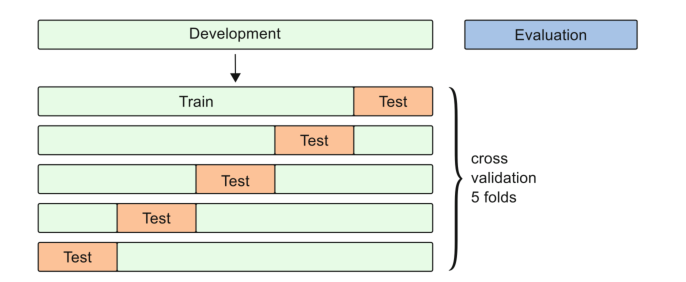
\includegraphics[width=0.8\textwidth]{img/cross-valid}
	\caption[Cross-validation splitting]{Splitting a dataset into development and evaluation data, with five folds for crossvalidation during system development.}
	\label{fig:cross-valid}
\end{figure}

Cross-validation folds also help avoid
overfitting and supports generalization properties of the system, so that when the
system is used on new data it is expected to have similar performance as seen with
the data used for development.

If available, a separate set of examples with reference annotation can be used to
evaluate the generalization properties of the fully tuned system. We refer to this set
as \textit{evaluation set}, and use it to evaluate how the system would perform on new data.

\newpage
